\documentclass[12pt]{article}
\usepackage[english]{babel}
\usepackage{natbib}
\usepackage{url}
\usepackage[utf8x]{inputenc}
\usepackage{amsmath}
\usepackage{graphicx}
\graphicspath{{images/}}
\usepackage{parskip}
\usepackage{fancyhdr}
\usepackage{vmargin}
\setmarginsrb{3 cm}{2.5 cm}{3 cm}{2.5 cm}{1 cm}{1.5 cm}{1 cm}{1.5 cm}

\title{LAB ASSIGNMENT 2}								% Title
							


\makeatletter
\let\thetitle\@title

\let\thedate\@date
\makeatother

\pagestyle{fancy}
\fancyhf{}
\rhead{\theauthor}
\lhead{\thetitle}
\cfoot{\thepage}

\begin{document}

%%%%%%%%%%%%%%%%%%%%%%%%%%%%%%%%%%%%%%%%%%%%%%%%%%%%%%%%%%%%%%%%%%%%%%%%%%%%%%%%%%%%%%%%%

\begin{titlepage}
	\centering
    \vspace*{0.5 cm}
    
\includegraphics[scale = 0.35]{City-Logo.jpg}\\[1.0 cm]	% University Logo
    \textsc{\LARGE CITY UNIVERSITY}\\[2.0 cm]
    \textsc{\lARGE COMPUTER SCIENCE AND ENGINEERING}\\[0.2 cm]
    \textsc{\lARGE ARTIFICIAL INTELLIGENT LABORATORY}\\[0.2 cm]
	\textsc{\Large CSE 418}\\[0.5 cm]				% Course Code
	
	\rule{\linewidth}{0.2 mm} \\[0.4 cm]
	{ \huge \bfseries \thetitle}\\
	\rule{\linewidth}{0.2 mm} \\[1.5 cm]
	
	\begin{minipage}{0.4\textwidth}
		
			\begin{flushright} \large
			\emph{STUDENT ID :} \\
			153402342\linebreak
			% Your Student Number
		\end{flushright}
	\end{minipage}\\[2 cm]
	
	{\large \thedate}\\[2 cm]
 
	\vfill
	
\end{titlepage}

%%%%%%%%%%%%%%%%%%%%%%%%%%%%%%%%%%%%%%%%%%%%%%%%%%%%%%%%%%%%%%%%%%%%%%%%%%%%%%%%%%%%%%%%%

\tableofcontents
\pagebreak

%%%%%%%%%%%%%%%%%%%%%%%%%%%%%%%%%%%%%%%%%%%%%%%%%%%%%%%%%%%%%%%%%%%%%%%%%%%%%%%%%%%%%%%%%

\textsc{\Large\section{MISSIONARIES AND CANNIBALS PROBLEM}}
\textsc{\Small 
\textbf{INITIAL STATE:}  IT IS THE STATE WHEN CANNIBALS AND MISSIONARIES ARE ON THE LEFT BANK OF THE RIVER WITH BOAT.I STATED THIS STATE WITH (MMM/CCC>R)}

\textsc{\Small
\textbf{FINAL STATE:}  FINAL STATE IS THEY ALL CROSS THE RIVER AND GO TO THE OTHER SIDE.
WHICH I STATED AS (0>MMM/CCC)}


\pagebreak
\subsection{STATE SPACE DIAGRAM}
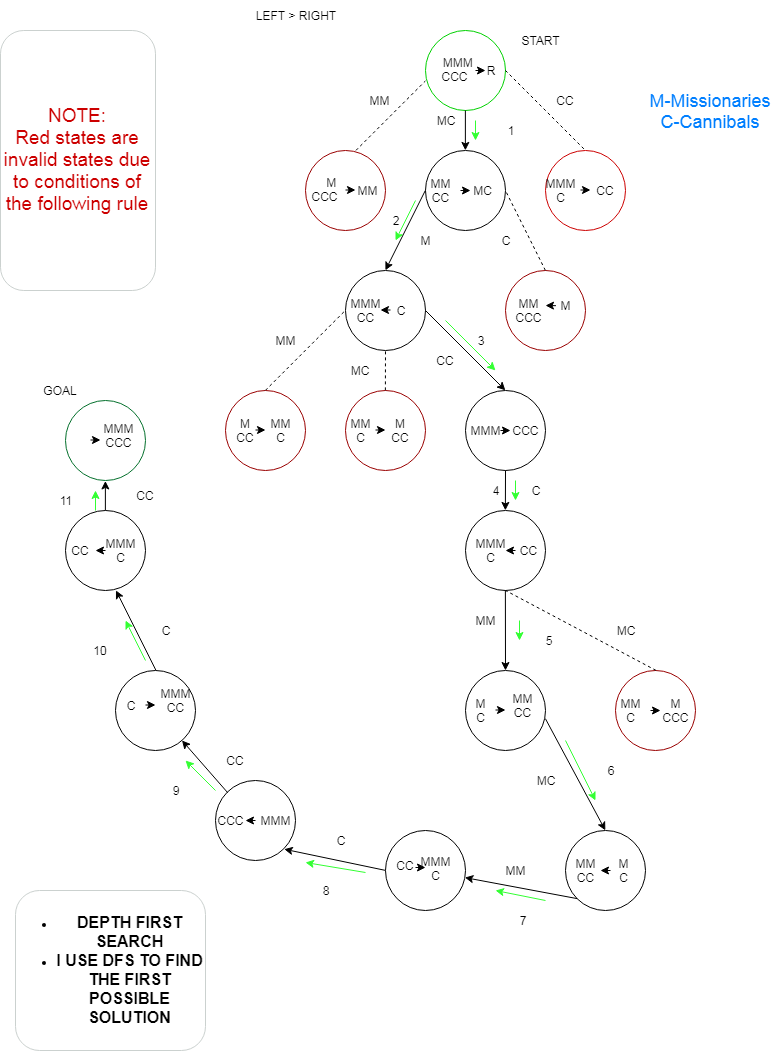
\includegraphics[scale = 0.38]{MMM CCC.png}

\begin{center}
 \caption{ Figure 1: STATE SPACE DIAGRAM}
    
\end{center}
\textsc{\Small TO SLOVE THIS PROBLEM, I USED DFS BECAUSE IT WILL TAKE LESS STEPS THAN BFS. }
\pagebreak

\textsc{\Large\section{LION,LAMB AND GRASS PROBLEM}}

\textsc{\Small 
\textbf{INITIAL STATE:} IT IS THE STATE WHEN LION,LAMBS AND GRASS ARE ON THE LEFT BANK OF THE RIVER WITH BOAT.(PlLG>R}

\textsc{\Small
\textbf{FINAL STATE:} FINAL STATE IS THEY ALL CROSS THE RIVER AND GO TO THE OTHER SIDE.WHICH I STATED AS (0>PlLG)}


\pagebreak
\subsection{STATE SPACE DIAGRAM}



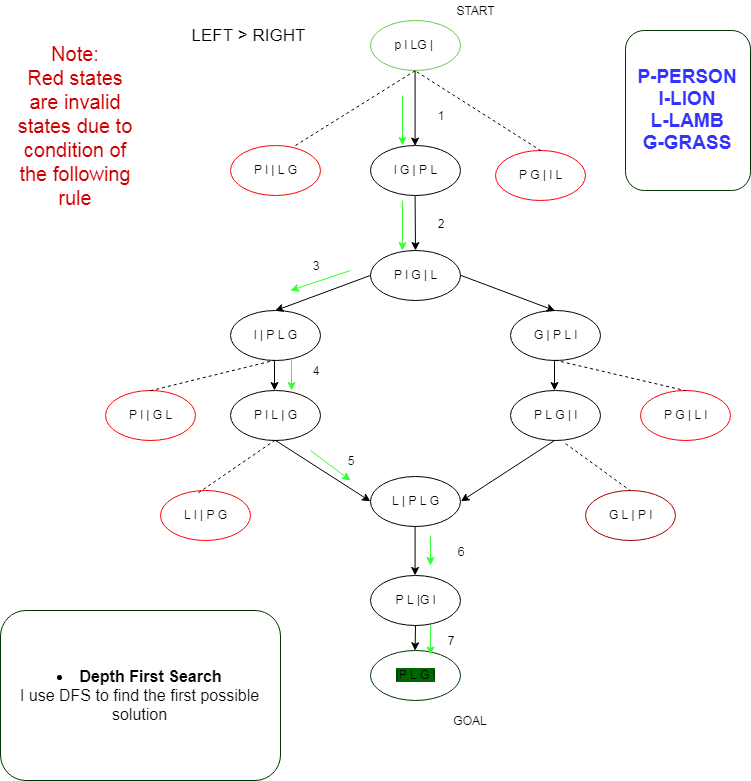
\includegraphics[scale = 0.30]{LION LAMB GRASS.png}\\[5.0 cm]

\begin{center}
 \caption{ Figure 2: STATE SPACE DIAGRAM}
    
\end{center}

\pagebreak

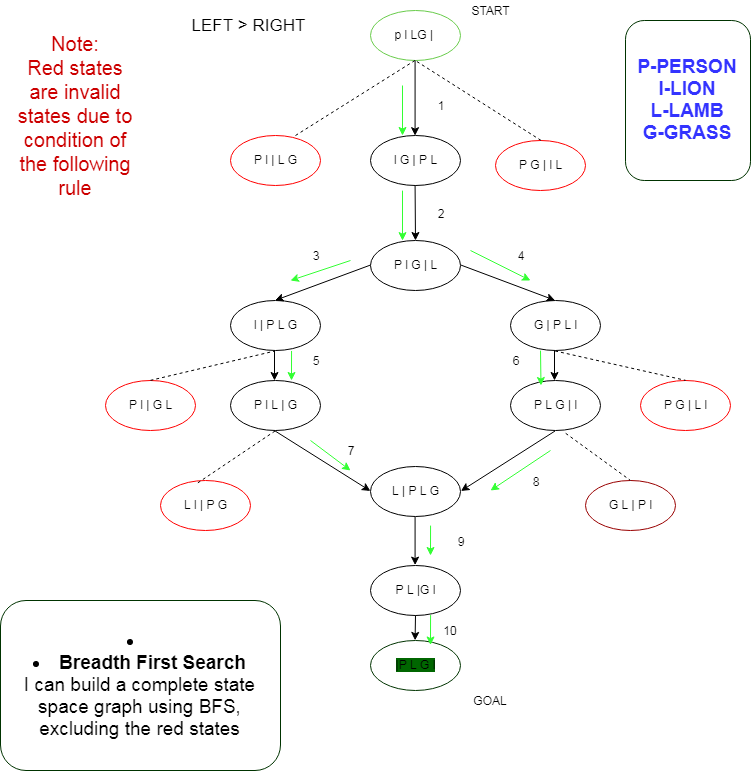
\includegraphics[scale = 0.30]{LION LAMB GRASS 1.png}\\[5.0 cm]

\begin{center}
 \caption{ Figure 3: STATE SPACE DIAGRAM}
 
    
\end{center}
\textsc{\Small TO SLOVE THIS PROBLEM, I USED DFS  BECAUSE IT IS OPTIMAL SOLUTION. }
\pagebreak


\end{document}
